\chapter{低血压与休克}

低血压(hypotension)系指成人肱动脉血压低于90/60mmHg的一种生理或病理状态。

根据发病速度,低血压可分为急性低血压和慢性低血压两大类:

1.急性低血压 短时间内,血压由正常或较高水平迅速明显下降,称为急性低血压。临床主要表现为晕厥与休克两大临床综合征。

2.慢性低血压 慢性低血压而伴有症状者,主要见于下列情况:①体质性低血压;②体位性低血压;③其他:如餐后低血压、高山性低血压等。

\section{41 慢性低血压}

\subsection{一、体质性低血压(原发性低血压)}

发病原因不清楚,常见于体质较瘦弱者,女性较多,可有家族遗传倾向。

临床特点:①多无自觉症状,仅在体检中偶然发现低血压,此种状况多无重要临床意义;②部分患者则有精神疲倦、健忘、头晕、头痛、甚至晕厥,或胸闷、心悸等类似心脏神经症的表现,但往往这些症状常由于合并某些慢性疾病或营养缺乏所致。

本症诊断主要依据:①低血压;②心或血管神经症;③无器质性疾病或营养不良的表现;④排除其他原因所致的低血压。

\subsection{二、体位性低血压(直立性低血压)}

从平卧位或下蹲位突然转变为直立位,或长时间站立时发生低血压(<90/60mmHg),或收缩压降低超过30mmHg,舒张压降低超过20mmHg,称为体位性低血压,严重者可以引起脑缺血症状或晕厥,若取平卧位,血压回升,症状可消失。

体位性低血压可分为原发性和继发性两大类:

\subsubsection{(一)原发性体位性低血压}

亦称直立性低血压、Shy-Drager综合征,是一种以自主神经系统功能失调为主的综合征。本病病因未明,多数学者认为可能是自主神经功能失调,导致血压控制异常;也有认为是自主神经原发性变性(尤其是交感神经系统所致)。

原发性体位性低血压临床特点:①起病隐袭,多在中年以后发病,男性多于女性,病程缓慢。②直立位时血压迅速而显著降低。③患者直立位时出现脑缺血症状,轻者头晕、眼花、乏力,多在晨起、登高、行走、活动或站立排尿时发生;重者立即发生晕厥,晕厥发作前无面色苍白,恶心、出汗、心悸等先兆。④有自主神经受损害表现:皮肤干燥、少汗或无汗、排尿障碍、夜间多尿与遗尿、阳痿、腹泻或便秘等。⑤本病可能为中枢神经系统疾病,可有躯体神经症状:说话缓慢、写字手颤或笨拙、步态不稳、共济失调;肌张力增高、腱反射亢进、发音困难,病理神经反射阴性。

本病诊断:①中年男性,于直立位时渐发头晕、眼花、眩晕甚至突然发生晕厥。②血压测定试验阳性;测量患者平卧位和直立位血压,每分钟1次,连续3~5次,血压下降>30/20mmHg为阳性。有学者认为,患者直立位收缩压较卧位下降50mmHg,舒张压下降20~30mmHg,有肯定诊断价值。③排除其他原因,包括血管迷走神经性晕厥、排尿晕厥、颈动脉窦过敏、严重心律失常等,可诊断本病。

\subsubsection{(二)继发性体位性低血压}

是继发于其他疾病或可查明原因,大致有:

1.神经系统疾病
脑干及其周围炎症、缺血、肿瘤等使血管运动中枢受累;脊髓疾病如脊髓结核、脊髓横断性损伤、脊髓空洞、多发性神经炎、多系统萎缩。

2.内分泌及代谢疾病
Addison病、慢性垂体前叶功能减退症、甲状腺功能减退症、重症糖尿病、嗜铬细胞瘤等。

3.心血管疾病
如重度主动脉瓣狭窄、重度二尖瓣狭窄、慢性缩窄性心包炎、梗阻性肥厚型心肌病、多发性大动脉炎、高原病等。

4.慢性营养不良
吸收不良综合征、重度贫血、慢性胰腺炎、严重肝病、恶性肿瘤、血液病、尿毒症、活动性结核病等。

5.药物性
某些降压药、血管扩张剂、镇静药等,如硝酸酯类、胍乙啶,α-受体阻滞剂等。

6.其他方面 妊娠晚期、久病卧床患者等。

继发性体位性低血压的病因甚多,下面仅介绍几种疾病:

1.慢性肾上腺皮质功能减退症(Addison病)
系由于各种病因使双侧肾上腺的绝大部分被毁致肾上腺皮质激素分泌不足的临床综合征。肾上腺皮质功能减退症临床上可分为急性及慢性,慢性又可分为原发性和继发性。病因见表\ref{tab13-1}。

\begin{longtable}{c}
 \caption{肾上腺皮质功能减退症的病因学}
 \label{tab13-1}
 \endfirsthead
 \caption[]{肾上腺皮质功能减退症的病因学}
 \endhead
 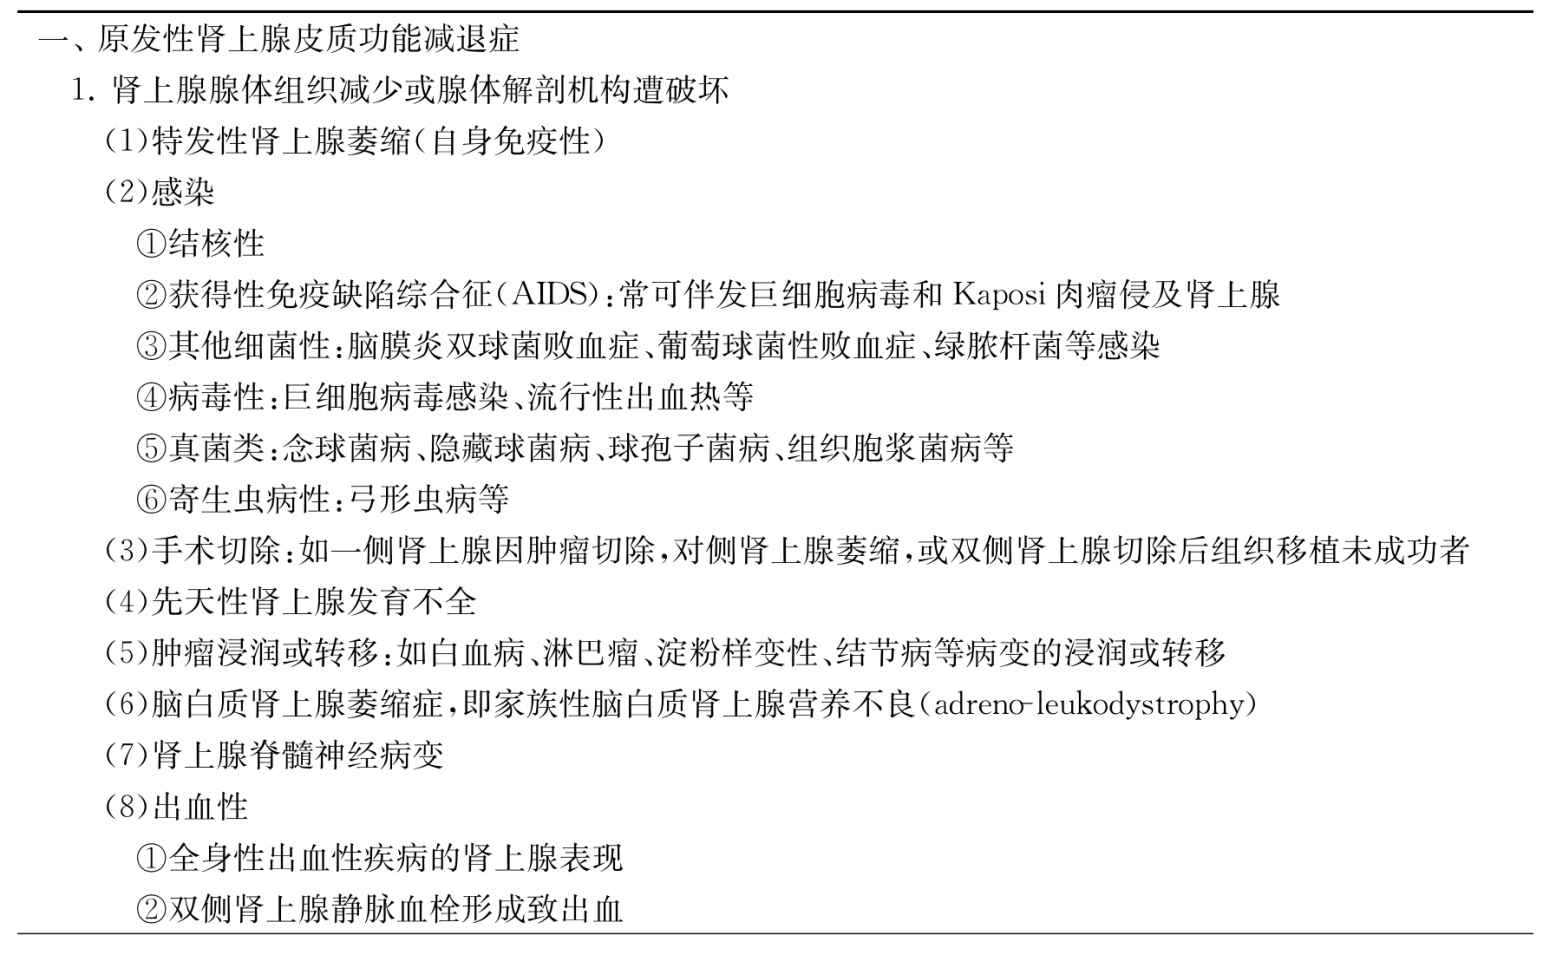
\includegraphics[width=\textwidth,height=\textheight,keepaspectratio]{./images/Image00087.jpg}\\
 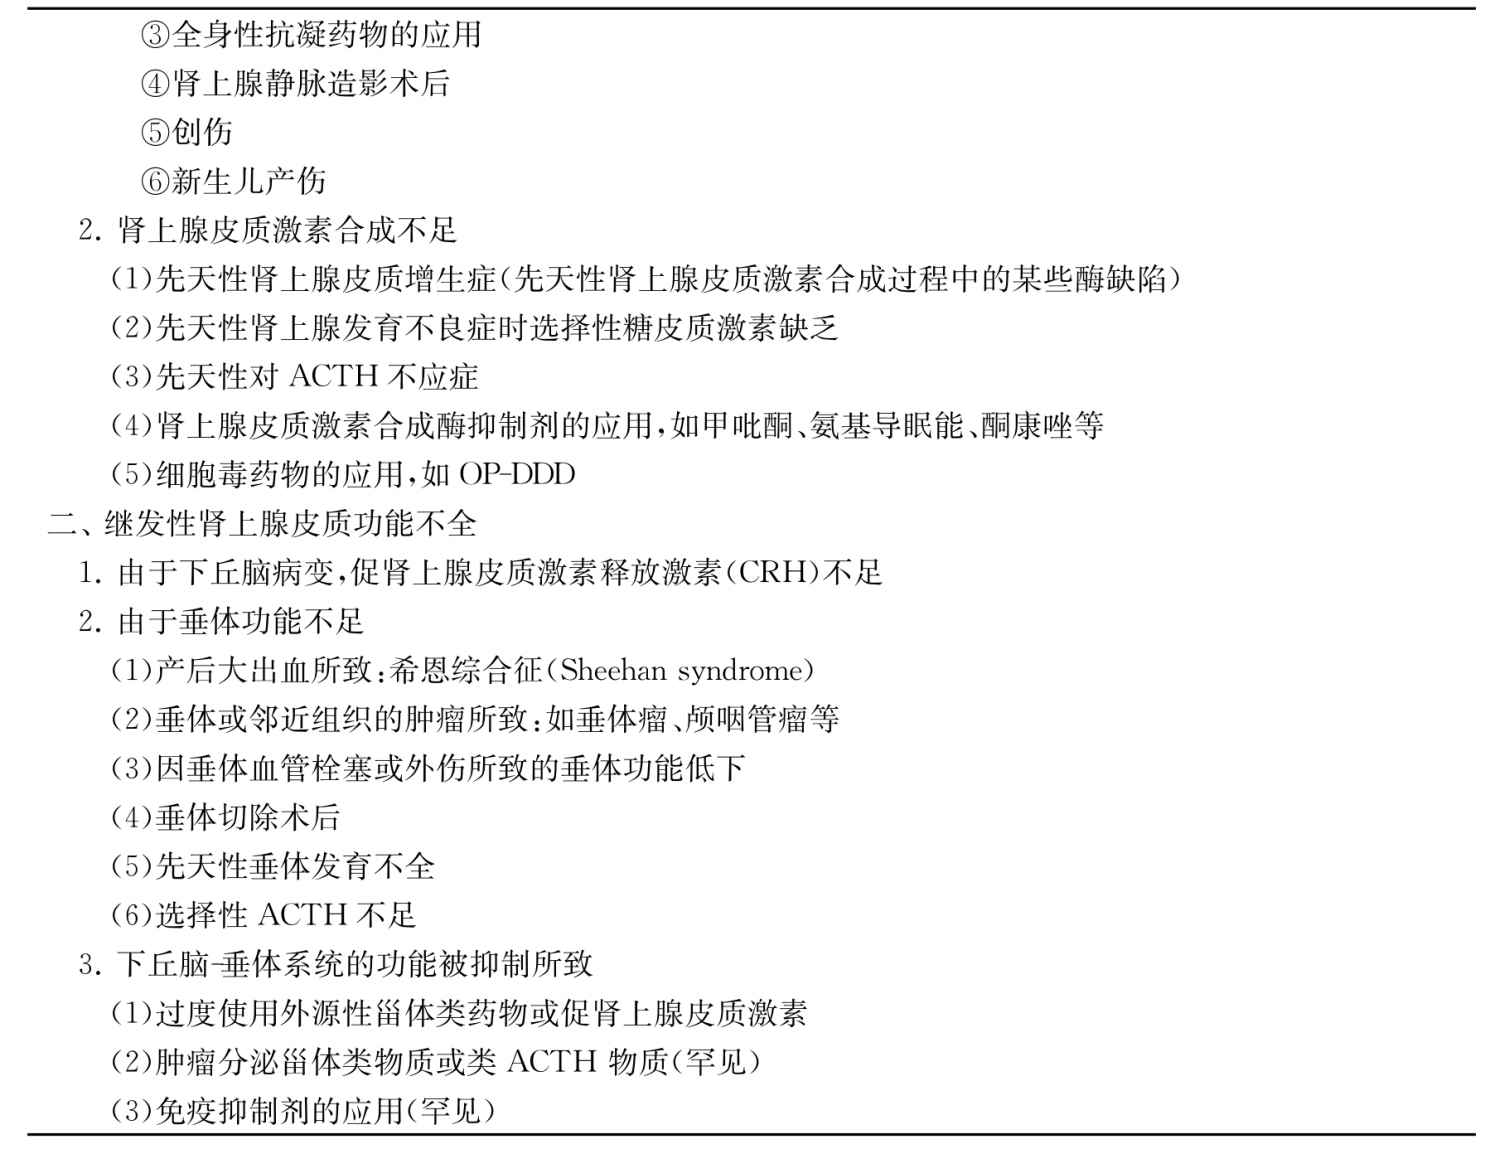
\includegraphics[width=\textwidth,height=\textheight,keepaspectratio]{./images/Image00088.jpg}
 \end{longtable}

原发性肾上腺皮质功能减退症的病因:①感染:肾上腺结核为本病常见病因,结核病灶破坏了肾上腺皮质和髓质;②自身免疫性肾上腺炎:双侧肾上腺皮质受损,约25\%患者血中可检出抗肾上腺的自身抗体;③少见其他病因:恶性肿瘤转移、淋巴瘤、白血病、淀粉样变性、双肾上腺手术,放疗破坏等,还有少见肾上腺白质营养不良症,属先天代谢异常疾病,本病也可有两型:儿童型及青年成年型。国外报道,自身免疫性慢性肾上腺皮质功能减退症占所有病例约80\%。近半数患者伴其他器官特异性自身免疫病,此称为自身免疫性多内分泌综合征,多见于女性(约占70\%)。

继发性肾上腺皮质功能不全的病因:①由于下丘脑病变,促肾上腺皮质激素释放激素不足;②由于垂体功能不足:如产后大出血所致希恩综合征(Sheehan
syndrome)、垂体或邻近组织的肿瘤、垂体血管栓塞或外伤、垂体切除、先天性垂体发育不全等;③下丘脑-垂体系统的功能被抑制所致,如过度使用外源性甾体类药物或促肾上腺皮质激素、肿瘤分泌甾体类物质、免疫抑制剂的应用等。

肾上腺皮质功能减退症的临床症状及特点见表\ref{tab13-2}:

(1)皮肤、黏膜色素加深及沉着,为本病最具特征性表现。皮肤暴露处、摩擦处、乳晕、瘢痕处色素加深更具明显,日晒后继续保持不退色;牙齿、舌部、颈、肛周等黏膜色素沉着明显。

(2)乏力为本病主要早期症状,其发生率高,程度与病情轻重成正比,应激状态下乏力症状加重。

(3)多系统及器官出现皮质激素不足表现:①胃肠道:纳差、喜咸食、胃肠功能紊乱;②神经精神系统:精神萎靡不振、疲劳,重者嗜睡、意识模糊、精神失常等;③心血管系统:低血压、部分有直立性晕厥、心脏缩小、心音低钝等;④代谢障碍:发生低血糖等;⑤肾脏:出现低钠表现;⑥性及生殖功能:性功能减退,男性阳痿,女性月经紊乱、闭经、阴毛及腋毛稀少或脱落;⑦合并全身疾病(如全身结核)或多器官自身免疫性疾病时则伴有相应疾病的表现。

(4)对感染、外伤、气候、劳累、情绪激动等各种应激的抵抗力差,易出现肾上腺危象。肾上腺危象为本病急骤加重的表现。其特点为:①常有应激状态(如上述感染、手术、分娩、创伤、过冷、过劳、失水或突然中断皮质激素治疗等);②临床症状加重:上述肾上肾皮质激素严重不足表现,如低血压或休克、严重失水、昏迷等;③抢救不及时,易休克、昏迷、死亡。

如怀疑或考虑本病,可进行下列实验检查。

(1)ACTH兴奋试验:最具诊断价值,Addison病者储备功能低下。

(2)24小时尿17-羟、17-酮类固醇测定:本病患者尿17-羟可接近正常。对本病有诊断意义。

(3)影像学检查:肾上腺区X线摄片、CT、MRI检查,可帮助诊断病因。

(4)血中嗜酸性粒细胞明显增多,血清钾增高、低钠、低氯、空腹低血糖或葡萄糖耐量试验曲线低平,均有助于诊断。

\begin{table}[htbp]
\centering
\caption{慢性肾上腺皮质功能减退症的症状发生率}
\label{tab13-2}
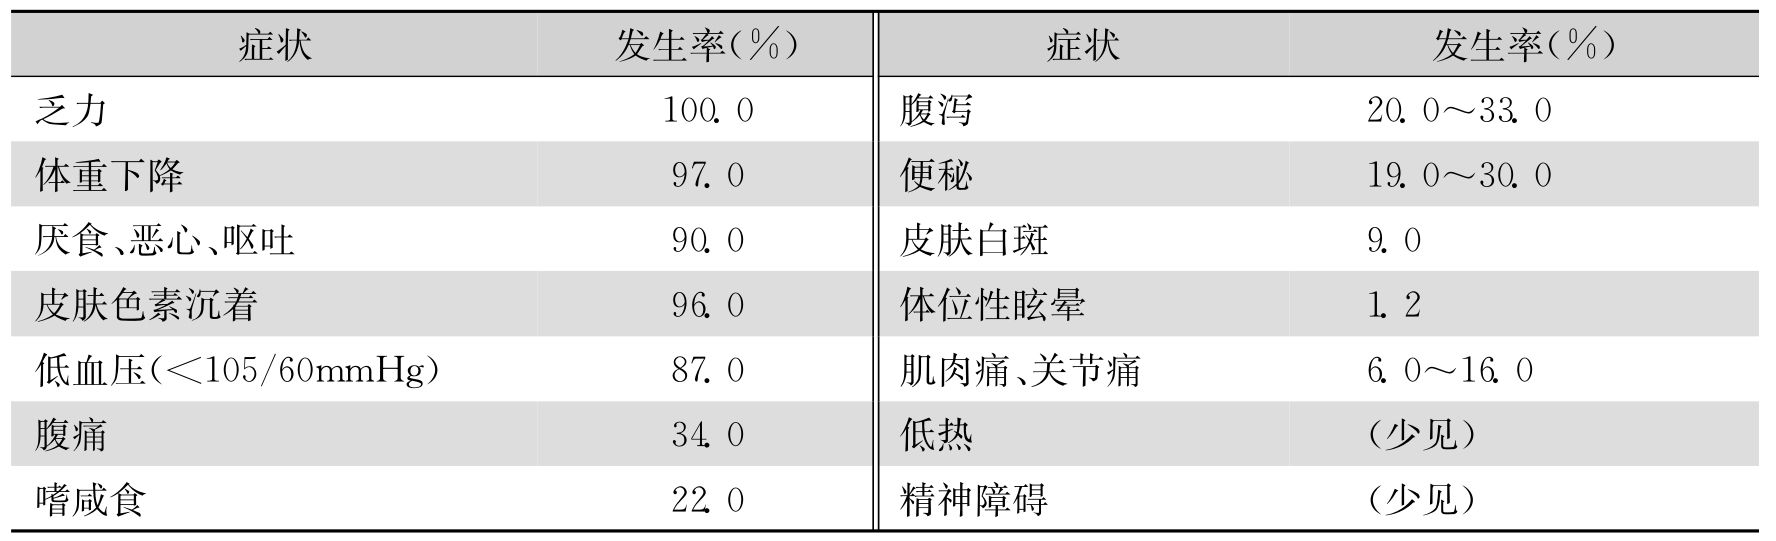
\includegraphics[width=5.91667in,height=1.79167in]{./images/Image00089.jpg}
\end{table}

2.腺垂体功能减退症
腺垂体功能减退症是指腺垂体(旧称垂体前叶)激素分泌减少,可以单个激素缺乏,也可以多种激素同时缺乏;腺垂体功能减退可以为原发(垂体病变),也可以继发(下丘脑病变,或下丘脑-垂体间的联系中断)。

腺垂体功能减退病因颇多,有:①垂体瘤:成年人最常见原因,也有其他恶性肿瘤转移至垂体;②下丘脑病变:如肿瘤、炎症、淋巴瘤或白血病浸润、结节病等;③垂体缺血坏死或纤维化:妊娠或产后的垂体功能减退症称希恩综合征,多发生前置胎盘、胎盘早期剥离、胎盘潴留、产后大出血;④下丘脑和垂体炎症与感染;⑤垂体瘤术后放疗及创伤,鼻咽癌放疗损伤下丘脑及垂体;⑥突然中断糖皮质激素;⑦垂体卒中、垂体瘤出血、瘤体增大压迫,临床呈急症危象。

本病临床特点:①本病多为女性(占95\%)20~40岁。②病情严重程度与垂体被毁程度有关。据临床资料,50\%以上腺垂体组织被破坏后才出现临床症状(轻度),75\%破坏时才有明显症状(中度),95\%破坏时可有严重垂体功能减退(重度)。③典型腺垂体功能减退主要表现为各靶腺(性腺、甲状腺、肾上腺)功能减退。

特别需要引起注意的是垂体功能减退性危象(简称垂体危象),在全垂体功能减退的基本表现下,在各种应激状态下均可引起或诱发垂体危象,临床上有各种类型表现:①高热型(>40℃);②低热型(<30℃);③低血压,循环衰弱型;④低血糖型;⑤中毒型;⑥混合型,突出表现为消化系统、循环系统、神经精神方面症状和表现,如高热、休克、恶心呕吐、谵妄、抽搐、昏迷等,甚至死亡。

本病需做实验检查,方可帮助诊断和判别诊断:

(1)腺垂体功能需检验其支配靶腺的功能来反映:①性腺功能测定:女性:血雌二醇水平降低,男性:血清睾丸酮水平降低或正常低值,精子量及质改变;②肾上腺皮质功能:24小时尿17-羟皮质醇,OGTT;③甲状腺功能测定;④腺垂体分泌激素测定。

(2)CT或MRI检查可辨别腺垂体及下丘脑病变,对非颅脑病变,也可用X线、CT及MRI或活检以判断原发病的病因。

本病需与多发性内分泌腺功能减退症、神经性厌食、失母爱综合征(与心理、社会因素有关)鉴别。

3.甲状腺功能减退症
甲状腺功能减退症简称甲减,是由于各种原因致低甲状腺激素血症或甲状腺激素抵抗而引起的全身性低代谢综合征,表现为黏液性水肿,成人原发性甲状腺功能减退症占成人甲减的90\%~95\%,其病因有:①自身免疫性甲状腺类;②手术或放射治疗破坏甲状腺;③过量碘摄入及抗甲状腺药物如锂盐、硫脲类等。

本病除有多系统及肌肉关节症状外,主要特征:①怕冷、易疲劳;②黏液性水肿伴高胆固醇血症;③低血压、心动过缓;④基础代谢率低;⑤血清甲状腺激素FT\textsubscript{4}
降低、TSH增高。

4.多系统萎缩症
多系统萎缩症是一类原因未明,临床表现为锥体外系、锥体系、小脑和自主神经等多系统损害的中枢神经系统变性疾病。

本病临床表现千变万化,包括锥体系、锥体外系、小脑和自主神经等多个系统的损害,最多见的组合为震颤麻痹合并小脑症状。其中41\%患者以自主神经障碍作为首发症状出现,主要表现为阳痿(男)、尿失禁(女)、直立性低血压、少汗、面色苍白、便秘等。高场强MRI对该病有较大的诊断价值。

本病需与帕金森病、家族性橄榄-桥脑-小脑萎缩、老年性直立性低血压鉴别(常由低血容量性、药物性、排尿性等低血压反应诱发)。

5.餐后低血压 餐后低血压(postprandial
hypotension,PPH)的定义为进餐后2小时内收缩压下降≥20mmHg或餐前收缩压≥100mmHg,而餐后收缩压<90mmHg;若进餐后收缩压下降幅度虽未达到上述标准,但超过脑血流自身调节能力出现低血压症状,如头晕、晕厥等,也可诊断为PPH。PPH是一种老年人常见的疾病,近年来与其相关的文献报道逐渐增多,发生机制尚不是十分清楚,一般认为,PPH的发生与压力感受器反射灵敏度下降、餐后交感神经活性反应下降及餐后体液改变等因素有关。

6.高山性低血压
平地人到海拔3500米以上地区时,可出现血压偏低。患者常有头晕、嗜睡、记忆力减退、全身无力、疲倦、纳差等。经过一段时间适应或离开高山地区,症状即可消失,恢复正常。

\protect\hypertarget{text00116.html}{}{}

\section{42 休克}

休克(shock)是一种危急的临床综合征,是由各种原因引起全身有效循环血容量急剧减少,导致全身微循环功能障碍,使脏器的血流灌注不足或严重障碍,引起缺血、缺氧、代谢障碍与细胞受损的病理生理综合征。患者表现有:①血压下降;②精神神经症状:头晕、乏力、神志淡薄或烦躁不安、嗜睡或昏迷等;③周围器官灌注不足表现:皮肤苍白、四肢湿冷、脉搏快而弱,甚至摸不到,少尿或无尿等一系列症状。

在临床上,休克按病因分类可分为:①低血容量(出血)性休克;②感染中毒性;③神经性;④过敏性;⑤心源性;⑥血流阻塞性;⑦内分泌性;⑧创伤性。有时同时存在2种或以上休克,临床上称为复合性休克,现把各种休克分述如下:

\subsection{一、低血容量(出血)性休克}

低血容量性休克包括出血性休克和体液丧失所致休克。出血性休克是指人体内较大的血管破裂出血,全身血容量急剧减少致急性贫血和循环衰竭的临床现象。体液丧失性休克往往与感染中毒、电解质紊乱联系或合并在一起,比如烧伤、急性胃肠炎、过度呕吐和腹泻、过度利尿、脱水,以及其他原因所致。本节主要是论述内科出血性休克。

\subsubsection{1.出血性休克常见原因}

(1)消化道出血:如消化性溃疡、各种原因肝硬化、胃炎或急性胃黏膜出血、胆道出血、胃肠道肿瘤等。

(2)呼吸道病变的大咯血:如支气管扩张、肺结核、肺癌等。

(3)心脏血管疾病,如重度二尖瓣狭窄的大咯血、主动脉夹层分离出血、肺高压、肺栓塞等。

(4)凝血机制障碍如血友病、白血病、再生障碍性贫血出血等。

女性宫外妊娠破裂出血虽属妇科,但内科也不应漏诊。

\subsubsection{2.出血性休克诊断}

\paragraph{(1)临床特点:}

①具有原发疾病相应病史及体征。②出血征象:依不同病因可表现为呕血或(及)便血、咯血,腹膜腔积血等;上消化道出血多为呕血及(或)黑便及暗红色便,下消化道出血多为便血;呼吸道及多数心脏病(二尖瓣病变、肺高压、肺栓塞、左心衰竭等)多为咯血,伴有心跳、气促、咳嗽、呼吸困难、发绀等;心包、胸腹腔急性出血需注意主动脉夹层破裂出血。③休克征象和急性贫血征:临床症状与出血量一般成正比,且与出血速度密切相关,一般情况下,成人短期内出血:小量(失血量800~1000ml),可有面色苍白、口干、出汗、烦躁、心跳、心率100
次/分、收缩压(SP)降至80~90mmHg;中量(失血量1200~1700ml),除上述症状加剧外,表情淡漠,四肢厥冷、尿量减少明显,心率100~120次/分、SP降至60~70mmHg、脉压小;大量(失血量1700~2000ml),面色苍白、四肢冰冷、表情极度淡漠或嗜睡、呼吸急促、发绀、心率>120次/分,SP降至40~60mmHg;极大量出血(失血量>2000ml),神志不清或昏迷,无尿、脉搏快而弱或扪及不到,SP降至40~30mmHg以下或测不到。另外,同等出血量情况下,出血速度愈快,则休克症状愈严重。

\paragraph{(2)辅助检查:}

根据病史或临床表现,选择有关检查,以明确出血量、出血病因,如做血常规(包括红细胞、血红蛋白、血小板、血细胞比容等)、各种腔镜(包括支纤镜、胃或结肠镜、胆道镜等),造影(支气管造影、血管造影等)、X线、超声、CT或MRI,以及心电图、凝血机制、腔膜穿刺等检查。

\subsection{二、感染中毒性休克}

感染中毒性休克是由于某一或多种致病菌及其中间产物通过某一或多途径进入血液循环,引起低血压及(或)多器官功能衰竭综合征。本类休克是内科最常见的休克类型,任何年龄均可罹患,治疗难度较大,近年来由于抗生素、皮质激素以及免疫抑制剂、抗癌化疗药物广泛应用,“二重感染”、院内感染、静脉输液/血被致病菌污染所致感染中毒性休克时有发生,致使病情复杂,更增加治疗困难。

感染中毒性休克诊断标准:

1.有明确感染灶(如局部化脓性感染灶)或呼吸道、肝胆道、泌尿道、胃肠道感染史或输血、输液(致病菌污染血或液体)病史。

2.全身炎症反应表现 起病急、畏寒/寒战、高热,伴急性病容、多器官功能障碍症状等。

3.休克血压
收缩压<90~80mmHg,或较原有基础收缩压下降>40mmHg,持续至少1小时,或靠输液及药物维持血压者。

4.周围组织灌注不足表现 少尿(<30ml/h)或无尿,神志急性障碍,面色苍白,皮肤湿冷、脉细数而弱等。

5.发现致病菌存在 血、尿、粪、脑脊液、病灶脓液培养致病菌阳性。

休克型肺炎、中毒性菌痢、暴发型流脑、流行性出血热均多见感染中毒性休克,内毒素性休克(由急性胆囊炎、急性梗阻性化脓性胆囊炎、急性肾盂肾炎所致)临床不少见,真菌(如念珠菌所致)败血症也可致感染中毒性休克,值得重视。

\subsection{三、神经源性休克}

神经源性休克(neurogenic
shock)是指在创伤、剧痛等的剧烈神经刺激下,引起血管活性物质(如缓激肽、5-羟色胺等)释放,导致周围血管扩张、微循环淤血、全身有效血容量突然减少所产生的休克。

内科神经源性休克可见于:①各种穿刺如胸腹腔,心包穿刺、骨髓穿刺、腰椎穿刺、血管穿刺等;②药物应用:过快静注巴比妥类药物(如硫喷妥钠),过量使用神经节阻滞剂降压药物;③麻醉意外、腔镜检查等。

剧烈的精神刺激(如恐惧、悲伤、兴奋过度等)所致面色苍白、肢冷、脉弱、血压下降、意识改变,这种一时性血管舒缩功能障碍,与休克在本质上是不同的,应加以鉴别。

\subsection{四、过敏性休克}

过敏性休克是由于抗原(致敏原)与相对应抗体相互作用所引起的一种全身性即刻反应,导致全身毛细血管扩张,循环血容量迅速减少而致心排血量急剧下降,危重者可危及生命。

可能引致过敏性休克的致敏原物质颇多,归纳为3类:药物性、动物性、植物性。进入人体的途径也有3种:①注射药物,如血清及造影剂;②口服某种/类药物或进食某些食物;③皮肤或黏膜被昆虫或毒蛇咬伤或接触植物。但在临床上,还是以注射药物引起的过敏性休克为最多见。可引起过敏性休克某些常见抗原物质见表\ref{tab13-3}。

\begin{table}[htbp]
\centering
\caption{可引起过敏性休克的一些常见抗原物质}
\label{tab13-3}
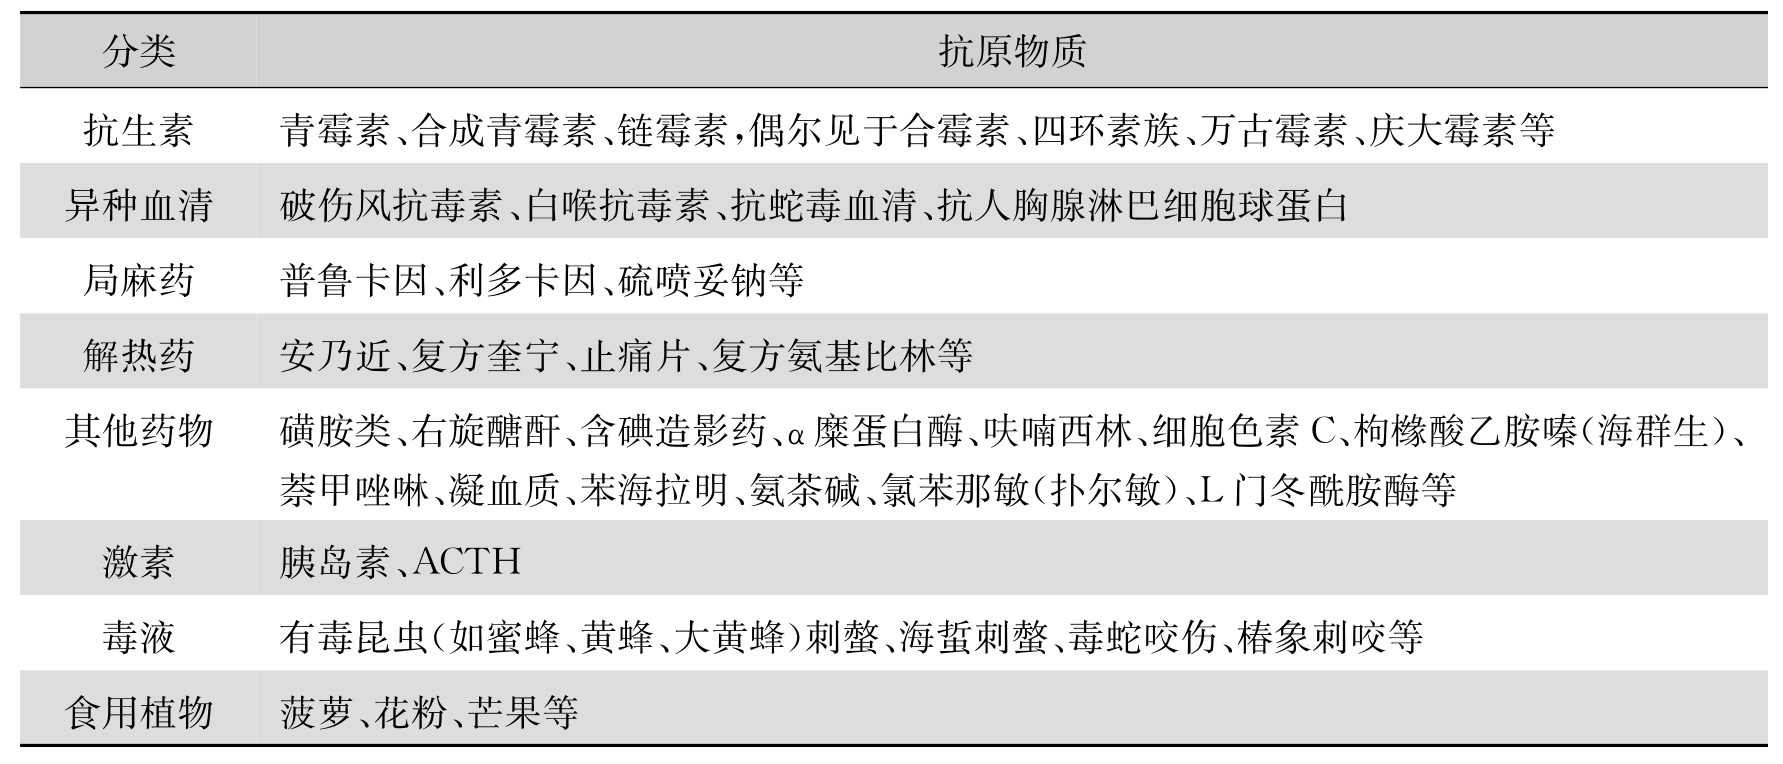
\includegraphics[width=5.9375in,height=2.54167in]{./images/Image00090.jpg}
\end{table}

过敏反应及出现过敏性休克除必须有致敏原物质外,在很大程度上取决于个人的所谓过敏体质。注射药物、血清引起过敏性休克,与剂量不一定呈正相关,但剂量过大而疗程过长,则可增加过敏性休克的机会。用药方式及途径与过敏性休克的发生有关系,注射(静脉、肌注,腔内注射)引起严重反应可能性最大,口服次之,局部用药(喷雾、贴剂、栓剂或滴眼、喷喉、口含、药膏外用等)引起严重反应可能性较少,但需注意个体差异。青霉素、头孢类抗生素可在长期用药过程中突然发生过敏性休克。

过敏性休克诊断要点:

1.有明确用药、进食动/植物、毒虫刺咬史。

2.有典型临床特点 ①如药物,尤其青霉素类过敏成人多见,儿童少见;②青霉素过敏性休克多属速发型、发作呈闪电样(5分钟内占50\%,半小时占10\%);③有喉头水肿/支气管痉挛引起症状;有循环衰竭、血压下降、休克等症状;有休克的神经系统表现等。

3.康复后有人认为可做被动转移过敏试验证实过敏性休克的致敏原,虽安全可靠,但操作复杂。

\subsection{五、心源性休克}

心源性休克(cardiogenic
shock)是指极严重心泵衰竭的表现,由于心搏出量严重锐减,导致血压下降,周围组织供血严重不足,重要器官进行性衰竭的临床综合征。心源性休克是心血管病最危重病征,死亡率极高(高达80\%以上)。

\subsubsection{(一)心源性休克病因}

大致分为下列几类:

1.心肌舒缩功能极度降低包括急性大面积心肌梗死(也包括急性右室心肌梗死等),急性暴发型及(或)重症心肌炎(如病毒、感染、中毒、风湿性心肌炎等);重症原发性或继发性心肌病(包括扩张型、限制型、肥厚型等),重度或晚期心力衰竭等,但以急性心肌梗死最常见。

2.心室射血障碍如大面积肺梗死,乳头肌或腱索断裂致急性二尖瓣反流,瓣膜穿孔致急性严重的主动脉瓣或二尖瓣关闭不全,室间隔穿孔等。

3.心室充盈障碍如急性心包堵塞,严重快速性心律失常,严重二尖瓣狭窄、左心房黏液瘤或人工瓣膜失控,球瓣样血栓堵塞二尖瓣口,心室内占位性病变等。

4.心脏直视手术后低排综合征。

5.混合型2种或2种以上原因,如急性心肌梗死并发乳头肌功能不全或断裂,或室间隔穿孔,其心源性休克预后差,死亡率极高。

\subsubsection{(二)心源性休克诊断要点}

1.具有明确的严重心脏病病史 比如大面积心肌梗死(梗死面积>40\%左心室面积)或严重病毒性心肌炎病史。

2.收缩压<80mmHg,或原有高血压者收缩压<90mmHg,或较基础压下降>80mmHg,低血压持续时间>0.5~1小时以上。

3.组织和器官灌注不足的表现 神志呆滞或不清,或烦躁不安,大汗淋漓,四肢厥冷,脉快而弱,发绀或呼吸促;少尿(<20~30ml/h),高乳酸血症。

4.排除其他原因所致血压下降 如低血容量、严重心律失常、剧烈疼痛、代谢性酸中毒、心肌抑制药物或血管扩张剂作用等。

5.主要血流动力学指标异常 动脉平均压(AMP)<65mmHg,心脏指数(CI)<1.8~2.0L/(min·m\textsuperscript{2}
),肺毛细血管楔压(PCWP)>18mmHg,左心室舒张末期压(LVEDP)>10mmHg,中心静脉压(CVP)>12cmH\textsubscript{2}
O。

\subsubsection{(三)心源性休克分型}

\paragraph{1.按病情严重程度分为}

轻度休克:神清、烦躁不安、面色苍白、出汗、口干、尿少、肢端轻度发绀或发凉、心率>100
次/分、收缩压≤80mmHg,脉压<30mmHg。

中度休克:表情淡漠,面色苍白、肢端发绀,尿量明显减少(<17ml/h),呼吸急促,脉搏细数,心率≥120次/分,收缩压60~80mmHg,脉压<20mmHg。

重度休克:神志不清、意识模糊、面色苍白、四肢厥冷、发绀,脉搏细弱,皮肤花斑样改变、极少尿或无尿(<100ml/24h),心率>120次/分,收缩压40~60mmHg。

极重度休克:昏迷,呼吸浅而不规则,发绀明显,四肢厥冷、脉扪不到或极微弱,心音低钝或单心音,无尿,收缩压<40mmHg或0,可有弥散性血管内凝血(DIC),多器官衰竭或死亡。

\paragraph{2.按微循环状态分类}

血管张力增高型:皮肤苍白、四肢厥冷、汗多、尿少、意识障碍严重。

血管张力减低型:皮肤较红、四肢较暖、汗少、尿略少、意识障碍较轻。

急性心肌梗死并心源性休克需与大面积急性肺动脉栓塞、急性心包炎/心包压塞、主动脉夹层分离、各种急腹症等鉴别。

\subsection{六、血流阻塞性休克}

血流阻塞性休克(blood flow obstructed
shock)是由于血液循环严重受阻,导致有效循环血量显著减少,血压迅速下降所致的缺血综合征。

血流阻塞性休克常见病因是起源于右心或大血管的急性血流受阻。如:急性肺栓塞(包括血栓性、脂肪性、气体、寄生虫、羊水等)、主动脉夹层、急性心包填塞、心房黏液瘤、腔静脉阻塞、心内人工瓣膜血栓形成或(及)功能障碍等。

下面重点介绍肺动脉血栓栓塞症及急性心脏压塞症。

1.急性肺栓塞是由于血栓栓子堵塞肺动脉主干或分支引起肺循环障碍的临床和病理生理综合征。深部静脉血栓形成(DVT)和肺栓塞(PTE)已成为国内外颇受重视的常见病,发病率高,死亡率很高。引起PTE的栓子可来源于下腔静脉径路、上腔静脉径路或右心腔,但大部分来源于下肢深静脉,特别是从腘静脉上端到髂静脉段的下肢近端深静脉(约占50\%~90\%),血栓栓塞可以是单一部位,也可以是多部位,病理检查发现多部位或双侧性血栓栓塞更常见,易见于右侧或下肺叶。

发生大块肺栓塞时,栓子阻塞肺动脉及其分支后,通过机械阻塞、神经体液因素和低氧作用,引起肺动脉收缩,导致肺循环阻力增加、肺动脉高压;右室后负荷增高、右室壁张力增加,右室扩大,可引起右心功能不全,严重者导致心排血量下降,进而引起体循环低血压或休克等。

急性肺栓塞诊断要点:

(1)临床表现缺乏特异性,但如能认真了解病史及进行细致的体格检查仍可做出初步诊断。①呼吸困难,占84\%~90\%,是急性肺栓塞最常见的症状;②胸痛,占40\%~70\%;③咯血,约占10\%~30\%,提示肺梗死发生;④惊恐、约占55\%,系低氧血症或胸痛所致;⑤晕厥,约占13\%,系大块血栓堵塞肺动脉,并发严重血流动力学障碍,引起脑供血不足所致;⑥咳嗽、干咳或少许白痰,占37\%。典型的“呼吸困难、胸膜性疼痛和咯血”三联症仅占28\%。

(2)体征:①低热、发绀;②呼吸系统征象;呼吸频率≥20次/分,可高达40~50次/分,可有肺部干湿啰音、胸膜摩擦音;③循环系统征象:窦速(心率>90次/分),可高达120次/分以上,可出现各种类型心律失常;肺动脉瓣区有喷射音或收缩期喷射性杂音;可有右心功能不全及心包积液体征。

(3)原有静脉血栓形成的症状和体征。

(4)实验室检查:①心电图:电轴右偏,S\textsubscript{Ⅰ}
Q\textsubscript{Ⅲ} T\textsubscript{Ⅲ} 型。T\textsubscript{Ⅱ、Ⅲ、aVF}
、V\textsubscript{1、2}
倒置,完全/不完全性右束支传导阻滞;②超声心动图、X线胸片、CT、MRI、核素显像(肺灌注/通气显像、肺动脉造影能做出定性、定位、确诊性诊断;③D-二聚体<500μg/L,基本可排除急性PTE或深部静脉血栓的诊断;>500μg/L,需做螺旋CT或肺通气灌注扫描,加以确诊。

急性PTE类型:①猝死型;②急性心源性休克型;③急性肺心病型;④肺梗死型;⑤“不能解释的”呼吸困难型。

2.急性心脏压塞症(急性心包填塞,acute cardiac
tamponade)系指心包腔内心包积液较快(几分钟或1~2小时内)增加而压迫心脏致使心脏舒张充盈障碍,心室舒张压升高,舒张顺应性下降,心输出量及全身有效循环明显减少的临床综合征。

急性心包填塞在内科临床上多见于急性渗出性心包炎、主动脉夹层分离破入心包、肿瘤性心包炎等,患者有心包积液征象而突然面色苍白、气促、血压下降或休克、脉搏细数、脉压减少、奇脉、颈静脉怒张、肝大、腹水、心浊音界迅速增大,高度提示本病,且应迅速解除心脏压塞症状(心包穿刺或外科手术排除心包积液)。

\subsection{七、内分泌性休克}

内分泌性休克系指某些内分泌疾病如慢性垂体功能减退症(希恩综合征),急、慢性肾上腺皮质功能减退症,黏液性水肿,嗜铬细胞瘤等,在某些情况下(如急性感染或出血)发生低血压或休克。

\subsubsection{1.慢性垂体功能减退症}

本病患者多因围生期大出血休克,使腺垂体大部分缺血坏死和纤维化,而致全垂体功能减退症,所有垂体激素均缺乏,但无占位性病变的表现。

\subsubsection{2.慢性肾上腺皮质功能减退症(Addison病)}

本病分为原发性和继发性,原发性者又称Addison病,继发性者由下丘脑-垂体病变引起。本病临床表现为全身皮肤色素加深、黏膜(齿龈、舌、颊部等)色素沉着,乏力、低血压及具有心、脑、肾、胃肠道、代谢、生殖系统症状,在各种应激状态下出现肾上腺危象,可伴休克。

肾上腺危象:①有诱因应激状态:各种感染、创伤、手术、分娩、过劳、寒冷、大量失水(包括大汗、呕吐、腹泻、失水),突然中断肾上腺皮质激素治疗等应激状态;②危象为Addison病急骤加重表现:恶心、呕吐、腹痛、腹泻、严重失水、血压下降、心率加快、脉细而弱、精神异常、高热、低血糖、低钠低钾血症,严重者休克、昏迷、死亡。

\subsubsection{3.急性肾上腺皮质功能减退}

本病是指肾上腺皮质功能急性减退、衰竭而表现有胃肠功能紊乱、高热、循环虚脱、低血压或休克、惊厥、昏迷等临床表现。

本病病因:①严重感染,如脑膜炎双球菌性败血症致双肾上腺出血,流行性出血热等;②原有Addison病,在各种应激状态下未加大应用皮质激素或停用皮质激素而诱发;③新生儿分娩损伤肾上腺出血所致;④其他原因,如长期大量皮质激素在应激下无增加剂量或停用皮质激素所致。其临床表现为高热、头痛、呕吐、腹泻、气促、发绀、全身瘀点/斑,可有惊厥、抽搐、休克、昏迷等。

\subsubsection{4.甲状腺功能减退症(简称甲减)}

甲减其病理特征是黏多糖在组织和皮肤沉积,表现为黏液性水肿(myxedema),成人原发性甲减占全部成人甲减的90\%~95\%;其主要病因:①自身免疫损伤,以自身免疫性甲状腺炎为多见;②手术或\textsuperscript{131}
I治疗后甲状腺受破坏;③碘过量;④抗甲状腺药物等。

甲减------黏液性水肿昏迷及休克,见于重症甲减。其临床特征:①多发病于冬季寒冷时;②多有诱因:除寒冷外,有合并全身性疾病、中断甲状腺素代替治疗、手术麻醉、镇静药物使用不当等诱因;③多表现为严重临床症状:低温(<35℃)、乏力、四肢肌肉松弛、反射减弱或消失、呼吸缓慢、心动过缓、血压下降、嗜睡、重者昏迷、休克,甚至死亡。

\subsubsection{5.嗜铬细胞瘤}

可以发生低血压,甚至休克,或出现高血压和低血压相交替的表现。低血压和休克发生原因:①本病分泌大量儿茶酚胺引起血管强烈收缩,组织缺氧、微血管通透性增加,血容量锐减;②大量儿茶酚胺引致严重心律失常或心力衰竭,致心排血量明显减少;若癌组织骤然发生出血、坏死,以致儿茶酚胺停止释放;③由于肿瘤组织主要分泌肾上腺素,兴奋肾上腺素能β受体促使血管扩张;④肿瘤还可以分泌舒血管肠肽、肾上腺髓质素等多种扩血管物质引起血管扩张;⑤本病在发生休克前常可有呕吐、腹泻、大汗淋漓、不能进食等症状,可产生低血压或休克。本病根据临床症状及体征,可进行血、尿儿茶酚胺及其代谢物测定,以及影像学(包括B超、CT、MRI等)检查而确定诊断。

\subsection{八、创伤性休克}

创伤性休克是指一些遭受严重创伤的患者,由于多种因素导致全身循环血量大减所引起的临床综合征,该病多见于外科临床,有人把其归纳为低血容量性休克范畴,因血容量锐减所致。

创伤性休克原因颇多,临床表现较为复杂,各个时期表现也不同:①临床上这类患者早期因骨折、挤压伤、大手术、烧伤等,使血浆或全血的丢失,加上神经刺激、组织损害,使损害部位的出血、水肿、渗出到组织间隙的液体不能参与有效循环,可使循环血量大减,出现休克;②由于损伤组织逐渐坏死及(或)分解产生如组胺、蛋白酶等,这些物质具有抑制血管的作用,引起微血管扩张和管壁通透性增加,使有效循环血量进一步减少,临床上出现休克或加重休克病情;③在组织损伤的过程中,往往可夹杂感染中毒以及心源性因素,也可出现休克。

\protect\hypertarget{text00117.html}{}{}

\section{参考文献}

1.何秉贤.体位性低血压的诊治现代概念.中华高血压杂志,2008,16(2):101-102

2.中华医学会内分泌学分会.甲状腺疾病诊治指南:甲状腺功能减退症.中华内科杂志,2007,46(11):967-971

3.The Surviving Sepsis Campaign Guidelines Committee including the
Pediatric Subgroup.Surviving Sepsis Campaign:International Guidelines
for Management of Severe Sepsis and Septic Shock.Crit Care
Med,2013,41(2):580-637

4.中华医学会心血管病学分会,中华心血管病杂志编辑委员会.急性ST段抬高型心肌梗死诊断和治疗指南.中华心血管病杂志,2010,38(8):675-687

5.中华医重症医学分会.低血容量性休克复苏指南.中华实用外科杂志,2007,27(8):581-587

6.Torbicki A,et al.The task force for the diagnosis and management of
acute pulmonary embolism of the European Society of
Cardiology.Guidelines on the diagnosis and management of acute pulmonary
embolism. Eur Heart J,2008,29,2276-2315

7.中华医学会心血管病分会肺血管组.急性肺血栓栓塞症的诊断治疗中国专家共识.中华内科杂志,2010,49(1):74-81

8.邹晓等.高龄老年餐后低血压的临床特点及防治策略的研究.中华老年心脑血管病杂志,2013,3(15):251-254

9.顾卫红.多系统萎缩的临床诊断与治疗.中国现代神经疾病杂志,2012,1(3),133-134

10.赵克松.创伤性休克新概念.中华创伤杂志,2005,25(1):29-31

\protect\hypertarget{text00118.html}{}{}

